\chapter{Introduction}
% 1st sect: GENERAL BACKGROUND: data environments evolve. data stream processing requires being accurate efficiently.
A problem occurring in nearly every application of machine learning is the challenge of handling evolving environments, a problem known as concept drift. Meanwhile, the domain of data stream processing proposes its own set of challenges, the main one being the ability to provide accurate predictions at any time despite large volumes of data and constrained time and memory resources. The combination of these two problems, the need to adapt to evolving data while meeting the systems requirements, is complex but common.

% there are lots of solutions to this so requirements are needed to select from them
Multitudes of approaches have been proposed to efficiently handle concept drift in stream processing systems, each with its own set of strengths. Therefore, to compare the applicability of these solutions, a set of requirements should be used as a starting point. A case study is presented for this purpose, and the solution is searched for given the set of identified assumptions and requirements.

% the context intro
The thesis at hand uses as context an ongoing research project, VesselAI, aiming to apply novel machine learning to the maritime domain. The domain in question is characteristic of the especially large volume of incoming sensor data and the slowness of vessel traffic in comparison. Additional context specifics include low-quality and heterogeneity of data and long delays in model feedback. 

% goal
The goal of this analysis is, given the project context, to find the most optimal system-level workflow for maintaining model accuracy. In other words, from the challenges identified in the VesselAI state-of-the-art analysis~\cite{D1.1}, the problem tackled is ‘ML model retraining is computationally very heavy: in environments where data evolves, it is urgent to use architectures that manage ML models in order to adapt to new data/tasks and retrain when necessary.' In addition to the suggested approach of lifelong learning, additional insight is gathered from the research fields of concept drift adaptation, deep learning optimization, MLOps and AutoML. This way, the literature gap of works addressing the maritime domain and automated model adaptation identified in~\cite{D1.1} is addressed.

% systems perspective
Traditionally, research addressing the problem of concept drift focuses on types of models able to adapt to a changing environment. This thesis can, from this perspective, also be seen as a systems approach to concept drift. If a model is taken as given, it is discussed how the system organization could ensure the model stays accurate. This perspective also aims to take into account the insight on best practices from big data systems. Especially the lessons of prioritizing simplicity and maturity are taken into account when searching for a system applicable to the real world. 

% 2nd section: RESEARCH Q'S, METHODOLOGY, RESULTS SUMMARY

% outline
% main question
% exact definitions of main question
% sub-questions
% note on methodology (literature based but not systematic, non-empirical)
% results summary

% comment: the sentence on the model is a little vague, tailored means that it is made for the case not just taken from somewhere else. I'm unsure what words to mention on the model here.

% research question
The main research question addressed in this work is the following:

\begin{center}
    Given the domain context and the models used, how to organize a workflow for efficient updating of the models in order to meet the demands posed by the use case?
\end{center}

 As further elaboration, by updating the model it is meant that the model parameters are changed. The domain context is the maritime domain, and the model used is assumed to be a deep recurrent neural network operating in batch mode. By efficient we mean especially the ability to handle large amounts of data by optimally utilizing high-performance computing resources. The main demand posed by the use case is that the accuracy of the models should either stay on a high level or ideally improve, which is referred to as \textit{model maintenance} in this work.

The complementary research questions considered as implications of the primary one are the following:

\begin{itemize}
    \item To which extent is it possible to optimize the training of the models?
    \item Which type of monitoring should be in place in the system?
    \item How much human intervention is required for maintaining the updating schemes; what are the possibilities of automating these workflows?
\end{itemize}

As a note on methodology, the investigation in its entirety is based on literature. Conducting a systematic literature review would be beyond the scope of this thesis, so only material directly relevant to the specific set of requirements is taken into account. Testing the various approaches in practice is also beyond scope; the empirical investigation of these findings is left to future works. This limits both the set of options considered to those already used in the problem domain and the evaluation to analyzing the thoroughness of existing evidence in literature.

% 3rd section: CHAPTER ROLES

The rest of this thesis is organized as follows:

Chapter 2 presents the necessary background knowledge to the reader. First, the phenomenon causing the need for efficient retraining, concept drift, is presented, alongside machine learning approaches aiming to cope with the problem. Then, as context, an overview of the general organization of a big data system is presented. Lastly follows an introduction to the maritime domain and the requirements of the case. Chapter 3 analyzes ways of enabling optimal model maintenance from three points of view. These viewpoints are data management optimization, speeding up neural network training and optimally timing the updates using concept drift detectors. In addition, it is discussed how certain these findings are given the quality and thoroughness of the literature used. The thesis is concluded with a discussion on the applicability of the results to similar problems from different domains.

\chapter[Overview of machine learning systems for the maritime domain]{Overview of machine learning\\ systems for the maritime domain}

% ingressi: mitä aiot rakentaa luvussa, mikä tulee esille, miksi se on tärkeää, mihin tällä kokonaisuudella pyritään

The general task of big data systems is that they should be able to handle vast amounts of data and from that be able to provide predictions in a timely manner. To position our problem of model maintenance in this larger domain, this chapter provides an introduction to the necessary background. First, background on deep recurrent neural networks and definitions for the relevant machine learning approaches are provided. Then, the entire big data pipeline and relevant design decisions are presented on an abstract level. Lastly, the requirements of the case used to compare the maintenance approaches are derived from the application domain description.

%online learing survey has lots of definitions that can be checked!
\section[Background on neural networks and machine learning approaches for model maintenance]{Background on neural networks and machine\\ learning approaches for model maintenance}

\enlargethispage{14mm}
% intro to rnn+dnn and stochgraddescent
\textbf{Neural networks} is a machine learning paradigm that takes inspiration from the human brain. The composition of a neural network is the following. The basic building blocks are neurons, collected in a layered architecture. A single neuron composes of weights and an activation function. The neuron takes weighted signals from the neurons of the previous layer and determines using the activation function which weighted value it passes on neurons connected to it on the next layer. \textbf{Deep neural networks} have more than one layer between the first and last layer, whereas, in \textbf{Recurrent neural networks}, there are not only connections to the next layer but also back-connections within the same layer~\cite{ben-nunDemystifyingParallelDistributed2019}. 

 Training a deep neural network means that the weights of the neuron-to-neuron connections are adjusted, usually using the algorithm called \textbf{stochastic gradient descent} (SGD)~\cite{ben-nunDemystifyingParallelDistributed2019}. The value of the final layer determines predictions to a learning task after the signal has passed through the entire network. The case study regarding marine traffic is assumed to use recurrent deep neural networks trained using the SGD algorithm.

% approaches opening paragraph: nonestablished terminology
The terminology presented next, regarding machine learning approaches, is somewhat indefinite. As the terms for various approaches have varying interpretations in literature, the definitions provided in the following paragraphs will define how these terms are used in this work.

% problem: concept drift incl. subtypes + delayed feedback
For the problem space addressed, the key term is \textbf{concept drift}. By concept drift we mean the case where the relation between the input
data and the predicted variable change over time~\cite{conceptdriftsurvey}. It is important to note that this does not mean the natural fluctuation occurring in data when sampling from a probability distribution, but when the probability distribution itself changes. As a simple example, fours repeating when throwing a dice would not be a concept drift, but changing the dice to one with multiple fours on it would characterize a drift. Concept drift can be further divided into types by the duration and scope of the drift. For duration, the terms \textbf{abrupt} and \textbf{gradual concept drift} distinguish cases where drift occurs over a short or a longer period of time~\cite{zliobaiteAdaptiveTrainingSet2010}. For scope, \textbf{global} and \textbf{partial} concept drift are used to distinguish between drifts occurring in all or only in a subset of the incoming data. As a further challenge in this domain, it is common that the correct answers for the prediction tasks are only available after some time~\cite{adaptivelearningsystems}, for which the term  \textbf{delayed feedback} will be used. 

% paradigms: what this is & is not
The terms related to machine learning approaches for dealing with concept drifts are the following. The approach regarding models capable of learning new tasks using previous training, such as a classifier being able to recognize unseen classes, is called \textbf{transfer learning}~\cite{iotsurvey}. \textbf{Lifelong learning} is a closely related field that explores the ability of models to adapt to new tasks, problems or environments, without losing the accuracy on previously learned tasks~\cite{lmlinneuralnets}. Transfer and lifelong learning, in these definitions, are out of the scope of this thesis. As for approaches that do not enable adjusting to new prediction tasks, \textbf{adaptive learning} refers to models able to adjust to concept drift~\cite{conceptdriftsurvey}. Somewhat synonymously, \textbf{continual learning} is used in varying definitions to refer to models able to operate accurately over longer periods of time. Summarized, both adaptive and continual learning could be used to characterize the problem of this thesis. However, only continual learning is used as it more accurately describes the problem at hand.

As for systems settings where machine learning is conducted, the following approaches are central. \textbf{Incremental learning} refers to cases where not all input data is available during training~\cite{giraud-carrierNoteUtilityIncremental2000}. As a subtype of this, in an \textbf{online learning} setting, data comes in as a stream one unit at a time and can be processed as such or in \textbf{batches}, meaning chunks of data~\cite{conceptdriftsurvey}.

% closing paragraph: what we are doing using this terminology
With the terminology presented above, our research challenge can be reformulated to be the following: The assumption is that there is a recurrent neural network trained on a small data sample. The aim is to enable retraining on large-scale data while mitigating concept drifts using continual online learning with batch processing. 

% add here description like this: The online learning setting under consideration is one
%where data can be buffered in batches using a moving window. So we do batch mode online learning.


\section[Best practices in big data systems design: organization and principles]{Best practices in big data systems design:\\ organization and principles}
% this is a long sect... a lot of stuff like lambdakappa and edgefogcloud can be omitted if necessary, they are more so nice to knows

% intro to subsection: why this is explained.
In the following section, the abstract components of a data streaming system are presented to clarify which parts are to be studied in the later chapters. Best practices are presented to have general guidelines for which traits to prioritize when comparing model maintenance approaches.

% list the components
% maybe add: this is an abstraction, feedback loops and multitudes of ways of implementation abstracted away
These parts in their operating order are data extraction, data preparation, data storage, model training, model evaluation and validation, model registry and model inference. It is assumed that the neural network used is readily developed and trained on a sample of data, as model development concerns, however non-trivial, are out of the scope of this thesis. For each of the system steps, the main task and general design decisions are presented next.

\textbf{Data extraction} is responsible for handling the incoming data. Usual forms of data are either web logs coming in from a server or IoT data from sensors that are often geographically distant from the data ingesting component.

The data to process is usually coming in as a stream. An important design decision to make is whether the data should be processed as such or in very small chunks, called stream processing, or by collecting data into larger chunks and processing those, called batch processing. The main advantage of using a batch representation is increased throughput, while stream processing allows smaller end-to-end latencies~\cite{mci/Feick2018}. 

To mitigate this trade-off between throughput and latency, a popular solution is called the lambda architecture. This reference architecture has a processing unit for both batch and stream data with the stream component, so-called speed layer, handling requests for the data not yet processed by the batch layer~\cite{beatingcap}. While this approach is widely accepted to solve the problem of handling highly voluminous data fast and mitigating human errors, the architecture has faced criticism for being redundantly complex and forcing code duplication~(\cite{questioninglambda},~\cite{uber},~\cite{facebook}). As an alternative, the kappa architecture has been proposed, only composed of a stream processor~\cite{questioninglambda}. This mitigates duplication but retains the trade-off with throughput and latency.

\textbf{Data preparation} encompasses the processes of data cleaning, transformation and feature engineering. Data cleaning refers to operations identifying and removing erroneous data, such as missing or impossible values. Data transformation and feature engineering are used interchangeably, both meaning processes that transform data into a format the models can process. A popular example of this is the mapping of plain text into word count matrices.

While the data preparation step is often overlooked in literature,
it is both a challenging and crucial part of the system, as preprocessing commonly takes up most of the total end-to-end latency of a machine learning system~\cite{adaptivelearningsystems}. As for systems design, the most relevant decision to make is whether to clean data before it is saved to the data storage or only when it is  needed for training. The main benefit with the first approach is that data only needs to be cleaned once, while the latter allows processing data for different models in different ways and retaining the data in its original form.
% the two approaches and their trade-offs need a ref...

\textbf{Data storage} is used to save the data needed for model training. The most often used storage methods are data warehouses and columnar databases. Here, it is important to note that storage times are generally short due to the volume of big data, usually the maximum being a few days (e.g.~\cite{uber}). The other extreme is one-pass processing, which means that the processed data is not stored at all.
% data archival needs a ref.

\textbf{Model training} means tuning the model parameters to fit the distribution of the incoming data in order to make accurate predictions from data coming in during inference.

% too short sentences, töksähtelee
The main design decision for this component regards infrastructure: distribution and parallelization. Centralized training, often run in a cloud data center, can run either on one machine or parallelized across multiple cores by splitting the model or the data~\cite{ben-nunDemystifyingParallelDistributed2019}. As the amount of data is large, high-performance clusters and modern general processing units are used to reach required latencies~\cite{iotsurvey}. The highest degree of distribution is called \textbf{federated learning} and refers to a setting where the training is conducted in the edge devices of a sensor network. This aims to solve the issues of moving privacy-sensitive data across the network and being adapting to the unique environments of each data source~\cite{iotsurvey}.

\textbf{Model evaluation and validation} refer to the stage where the model is tested; usually various model metrics such as accuracy for classifiers and error statistics for regression tasks are checked~\cite{iotsurvey}. These numbers can also be compared against other models, possibly models already in operation~\cite{googlemlops}. Also, testing different data sets and checking compatibility with the rest of the system is conducted at this stage~\cite{googlemlops}.
\enlargethispage{7mm}

In addition to testing, models are also optimized for the infrastructure that they are being deployed on. This can include, for example, various performance optimizations, or in the case of constrained memory, model compression~\cite{iotsurvey}.

\textbf{Model registry} is a centralized storage for the trained models. As trained models do not require a lot of memory, this stage has little complex design matters.

\textbf{Model inference} refers to the model being in production and answering application requests.
The most important design decision to make for this component is where to deploy the models. The options are a centralized cloud data center, the sensor network edge devices, or fog, which refers to any devices between the edge and the cloud~\cite{fogsurvey}. The main advantages of the distributed approaches are, similarly to distributed training, reduced network latencies and better privacy~\cite{szeEfficientProcessingDeep2017}.

The components presented above are summarized in Figure~\ref{simplepipeline}.

% the figure is too small... -> not very readable
\begin{figure}[hb]
%\begin{figure}[tbh] t= top, b = bottom, h=here
\newline
\begin{center}
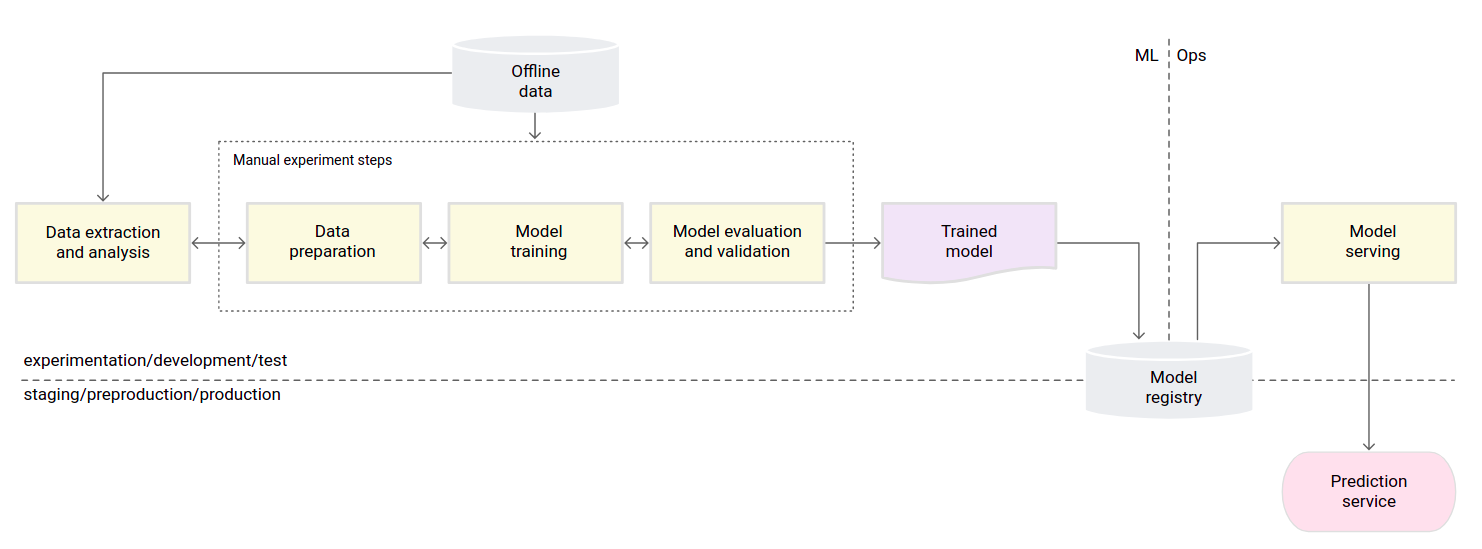
\includegraphics[width=1.0\columnwidth]{simplegoogle.png}
\caption{Abstract components of a big data analytics system~\cite{googlemlops}.}
\label{simplepipeline}
\end{center}
\end{figure}

% model updating within inference, thesis concerns (iotsurvey has monitoring stuff if needed)
% maybe add: this is like CI and CD but CT=continuous training (from~\cite{googlemlops})
The concerns of this study are within the step of model inference. Due to the evolving nature of data, this step requires a scheme for maintaining the accuracy of the model. For this purpose, a retraining pipeline, model monitoring system and a retraining trigger need to be in place. From these parts, especially the retraining, monitoring and trigger components are investigated. This general abstraction of the updating scheme, highlighted with the focuses of this thesis, is presented in Figure~\ref{triggerpipeline}.

% the figure is too small... -> not very readable
\begin{figure}[ht]
%\begin{figure}[tbh] t= top, b = bottom, h=here
\ \newline
\begin{center}
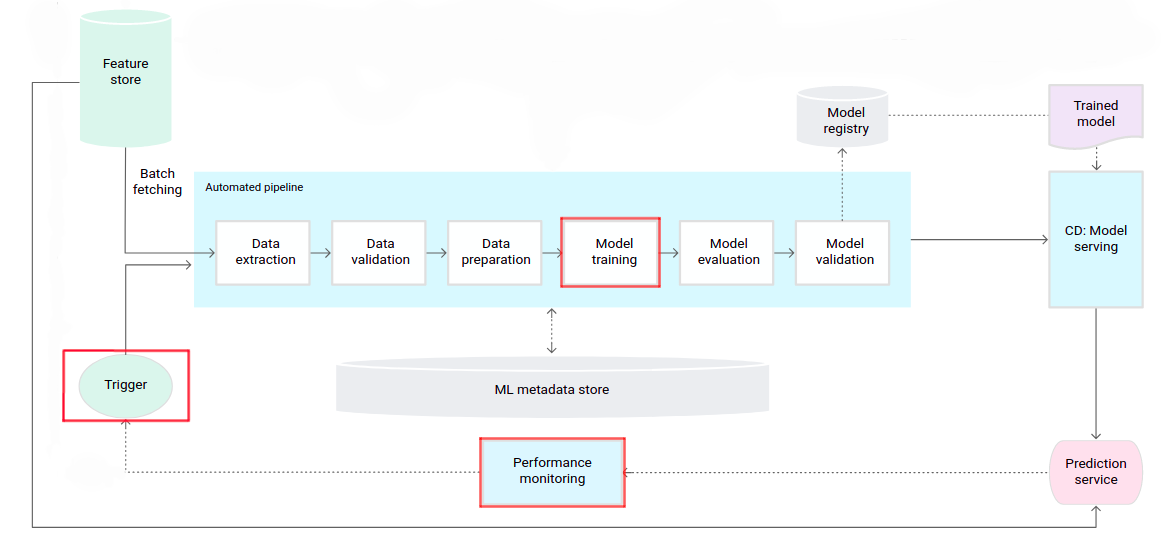
\includegraphics[width=1.0\columnwidth]{paivityssykli.png}
\caption{Automated retraining workflow, simplified and highlighted by the author~\cite{googlemlops}.}
\label{triggerpipeline}
\end{center}
\end{figure}


% best practices + automation: mlops and automl
Lastly, the most important best practices in building a successful big data system are the following. These are combined lessons learned from the most mature big data systems of our time, Google MillWheel~\cite{millwheel}, Facebook~\cite{facebook}, Twitter storm~\cite{storm@twitter} and the Uber system~\cite{uber}. As the most important was deemed ease of using and improving the system, which includes modularity and simplicity. The two other principles named important across these systems were scalability and resiliency, the latter including tolerance to failures and exceptions. 

\enlargethispage{-7mm}
As an important part of system-level ease of use was named the fact that human intervention should be minimized. This is a general trend in big data systems, as in other fields of technology. The field of MLOps aims to, similarly to DevOps, unify machine learning system development and operation, which means that automation and monitoring are advocated~\cite{googlemlops}. Automation and minimizing human intervention is the topic of study in the field of \textbf{AutoML}~\cite{celikAdaptationStrategiesAutomated2021}.


% section conclusion: what was said & how it relates to whats to come
The principles of simplicity, scalability, resiliency and degree of automation will be another point considered when choosing the most appropriate model updating workflow: from the promising-seeming options encountered, the goal is to find one that would meet these best practices as well as possible. From the full systems perspective, this goal means handling one part of the process, model updating, as successfully as possible. Seen this way, our goal is the means to the ends of setting up a full, efficient data processing pipeline.

\section[Context and requirements from the maritime domain]{Context and requirements from the maritime\\ domain}

% why this section: we need to know the context to know the requirements to choose the right approach 
Lastly for the background, this section introduces the maritime domain and elaborates its specialties that are used to find the most optimal model maintenance workflow.

% maritime is global
The domain of application, maritime, differs in a few ways from others from the point of view of a sensor-based machine learning system. The most obvious difference is its global nature: while other spatial domains such as smart cities also have to take geographical distribution into account, the maritime domain is special as it encompasses all of what the earth's surface is mostly covered by: the seas. 
% maritime is extreme heterogeneous data

As another characteristic, equally to the area that is operated in, the amount of traffic is large, resulting in data volumes exceeding even what is conventionally noted as big data. Due to international regulation, vessels have to send update signals of their status from every few minutes to every two seconds, depending on their speed and course~\cite{maritimeinformatics}. With approximately 100 000 ships sailing the world oceans daily~\cite{maritimeinformatics}, billions of messages are sent each day. To this exceptional amount of data we refer to as \textit{extreme-scale data} in this work. In addition to this, in order to provide valid maritime intelligence, other types of data such as geographical information and weather reports are needed~\cite{D1.1}. Therefore, the data is not only highly voluminous but also heterogeneous, coming in both static and dynamic forms at different velocities.

% lack of speed in terms of vessels
Added to scale, another specific of this context is speed, or more specifically, the lack of it. Depending on the size and type of the vessel, it takes from minutes to an hour to change course. This means that for machine learning services in this domain, the acceptable end-to-end latencies are measured in seconds, even minutes. This differs greatly from other sensor system applications, where latencies are usually measured in the order of hundreds of milliseconds (e.g.~\cite{facebook},~\cite{edgelatency}). This means that striving for instant response times is redundant, even of detriment, as prioritizing latency inevitably would introduce the need to make compromises in other respects.
\enlargethispage{7mm}

% AIS intro
The main data source, the status signal data sent by vessels, called \textbf{automatic identification system} (AIS) data, also has its specialties. AIS is a form of sensor data and has two types: static messages containing information such as name, destination and ship characteristics, and dynamic messages with information on the vessels' location, speed, heading and rate of turn. The challenge with AIS data is both its highly fluctuating reporting intervals and especially its unreliability.  Things such as manually written destinations, faulty timestamping, lack of universal identifiers, misreported locations and even illegal traffic camouflaging their operations make identifying and correcting erroneous data difficult and computationally expensive. In addition to faults in the data itself, the traffic system adds another layer of error: for example, in busy areas, large parts of messages can go lost because of overloaded receivers, and vessels sometimes shut off their transmitters in fear of smugglers~\cite{maritimeinformatics}.

% pilots
The project studied, VesselAI, aims to provide the following four pilot services to users: route forecasting for traffic monitoring and management, design of optimal ship energy systems, operating autonomous ships in short-sea transport and weather-optimized routing for long-distance voyages. In addition to this, the more abstract goals are to find a system that is suitable for both managing extreme-scale data and enabling the models to run in production over extended periods of time. The goal is also to fully utilize the most modern high-performance computing infrastructures and develop new machine learning methods~\cite{D1.1}. The emphasis with these models is on deep learning, which is also the focus of this thesis.

% requirements derived from above
With this context and goal specification in mind, the following system goals and challenges can be stated. The general goal is to provide accurate predictions, not in an instant but still in a time-constrained manner. Two main challenges arise from the combination of the context and required services that most pressingly need to be addressed to reach this goal. Firstly, the nature of data used sets high demands on the training part of the workflow: storage, preprocessing and training. Secondly, given the environment of operation, concept drift identification poses a challenge. As data quality is low, distinguishing drift from noise is hard, especially as it can be expected that the drifts will be more of the gradual type; abrupt drifts will likely be encountered only within subsets of the data. The time spans of vessel operating mean that the prediction correctness is known only after days, which means that the problem of delayed feedback is very present in the domain.

How to deal with these challenges in order to build a system able to meet its requirements is the primary topic of inspection in the following chapters.

%outline:
% 1st paragraph: maritime specifics: geo distr, volume, vessel slowness
% 2nd paragraph: data is heterogeneous and error-prone
% missing data due to lots of traffic -> receivers dont take in everything. senders turned off bc smuggling

% 3rd paragraph: pilots n abstract aims
% the project
%	the pilots I-V: what each one aims for
%		these ml problems are difficult
%	abstract aims
%		deal with extreme scale data
%		facilitate continuous learning
%		utilize modern HPC

%data thoughts
%		static and dynamic, fast and slow paced
%			examples: map data, weather data, sensor data
%	many models only need a small fraction of the data


% combine these: the requirements.
% we want accurate solutions to hard problems not instantly, but it should not take forever either
% security is no obstacle
% obstacles to reach this
% there's a big need for data preprocessing (emphasis on workflow efficiency)
% concept drift is gradual large scale abrupt only in subset of data (napa example: vessels start anchoring somewhere)
% concept drift: noise vs drift is hard to distinguish bc error data
% correct labels to data come delayed, talking about days to couple weeks. hard to get labels also is possible. mention delayed labels


\chapter{Analysis of efficient updating cycles for batch learning}

In this chapter, solutions to the problem of efficiently updating the models are analyzed. Specifically, we assume that the starting point is a recurrent neural network trained on a small sample of input data and that the environment faces occasional concept drifts, mainly of global and gradual, or abrupt and partial type.

The challenges to address with enabling efficient update cycles are ensuring and monitoring data quality, enabling training scaling to larger data sets through optimized training and finding the optimal times when the model should be updated. The approaches for addressing these problems are discussed next.

\section[Prerequisite for retraining: efficient data management]{Prerequisite for retraining: efficient data \\management}

What differentiates machine learning systems from traditional software systems is that the quality of the model does not only depend on the machine learning algorithm used but also on the data it was trained on~\cite{polyzotisDataLifecycleChallenges2018}. Therefore, there need to be mechanisms ensuring that the data is of high quality during the updates, which is referred to as \textbf{data quality assurance} in this thesis. Secondly, there needs to be knowledge on which data, transformed and cleaned in which ways, was used. This problem is known as \textbf{data versioning}.

\enlargethispage{7mm}
The following aspects need to be taken into account when considering data quality assurance. For data cleaning, it is important to ensure that the data format is consistent, which means that the data the model was trained on should be in the same format as during inference~\cite{polyzotisDataLifecycleChallenges2018}. It is also important to consider the model used when creating the cleaning processes: as some data noise impacts model performance more than other noise, the most optimal cleaning scheme needs to take into account the specifics of the model~\cite{renggliDataQualityDrivenView2021}. As for the quality of the testing data used after training the model, the same test data set should not be used too many times, as that can lead to the model predicting perfectly on the test data set but poorly on other sets, a phenomenon known as over-fitting~\cite{renggliDataQualityDrivenView2021}.

In the inference stage, it is known that there sometimes occur unexpected changes in the data format, which may decrease model performance without system failures. For these data errors, there needs to be an alerting system that thoroughly validates the incoming data and triggers a warning in case the data format has changed unexpectedly~\cite{polyzotisDataLifecycleChallenges2018}.

For data versioning, the general goal is to keep track of which data was used and how it was transformed before training while avoiding keeping copies of data in memory~\cite{maddoxDecibelRelationalDataset2016}. The usage of traditional version control such as git is unsuitable for data versioning as it does not take into account the size and structuredness of data files. For instance, to make changes to a file using git, the user has to copy the data file to their local machine, which is infeasible in cases of large files~\cite{maddoxDecibelRelationalDataset2016}.

Works aiming at creating data-tailored versioning systems, such as Decibel~\cite{maddoxDecibelRelationalDataset2016} and OrpheusDB~\cite{huangEffectiveDataVersioning2019}, aim to minimize storage costs for each data version and the time it takes to retrieve a version from memory. The main advantages are saved memory and no need to preprocess the same data many times. Another approach, implemented by the Shibsted System~\cite{vanderweideVersioningEndtoEndMachine2017}, saves all information regarding the data source and its processing into a tuple and saves the preprocessed data into a file path hashed from this metadata. This approach is significantly simpler than the previous one.

Given the case requirements, it is likely that a batch of data is needed in the preprocessed format only for a small time window needed to train all models using that data. Therefore, storing the preprocessed version of the training data for longer is likely to be redundant and memory-consuming, especially due to the extreme scale of the data. However, part of the data will be needed again in the preprocessed format: in case there are indications of data errors, the data used needs to be checked manually. Therefore keeping the original data, identifiers to it and the preprocessing used is necessary to enable reproducibility for all model versions in production. This simple identifier-based versioning is implementable using existing machine learning lifecycle management tools, such as MLflow~\cite{mlflow}.

Summarized, to enable operating a successful machine learning system, data needs to be versioned and of high quality at every stage of the system: training, testing and inference. These should be assured using identifier-based versioning and thorough data validation.

\section[Optimizing retraining: parallelization and approximation in deep neural network training]{Optimizing retraining: parallelization and \\approximation in deep neural network training}

% not mentioned but maybe should: in neural net processing memory access, data moving, and multiply-accumulate ops are the most expensive

% not mentioned: why the highlighted approaches were highlighted (seem most mature for training recurrent networks, a lot of approaches optimize inference and convolutions for cnns)

The goal of optimized retraining from the perspective of concept drift adaptation is that the more often model updates can be executed, the better they can keep up with environment changes with stationary or increasing model accuracy. The aim is to minimize the cost of an update cycle so that update frequency can be increased. As deep neural network training can take from hours to days, even weeks~\cite{szeEfficientProcessingDeep2017}, reducing training costs is crucial: update cycles of this time span would, for instance, make the weather-based routing services outdated already before their training is finished.

% assumption of feeding more data, should this be questioned?
The research question for this section is an implication of the main one: how can the retraining time of recurrent neural networks be reduced? It is assumed that the model is retrained on a cloud data center as moving data to the cloud requires time spans measured in hundreds of milliseconds~\cite{edgelatency}, which is a short time given the acceptable response times (up to minutes) of the maritime intelligence case. Additionally, the model is assumed not to be retrained from scratch but by feeding the previous model with new data. Assuming these, the approaches of neural network parallelization and reduced precision networks will be discussed next.

\textbf{Distribution and parallelization}

Distributed neural network training allows increasing utilization of the used hardware and therefore reduces the training time of the network. The methods to implement parallelism can be coarsely divided into two types: data and model parallelism~\cite{ben-nunDemystifyingParallelDistributed2019}.

Data parallelism means that parallel training is conducted by dividing the incoming data batch into parts and executing the training with those on different cores. As the de-facto neural network training algorithm, SGD, is sequential by nature, the way of enabling data parallelism is by using the so-called mini-batch SGD, where the training on individual mini-batches can be distributed~\cite{DBLP:conf/icml/LeNCLPN11}. The common way of introducing more parallelism is through increasing the mini-batch size, which is proven to reduce training times~(\cite{shallueMeasuringEffectsData2019},~\cite{smithDonDecayLearning2018}). However, increasing the batch size introduces a trade-off known as the generalization gap~\cite{hofferTrainLongerGeneralize2018}: the accuracy of the model generally decreases when using larger mini-batches. The main research topic in data parallelism is therefore to find techniques for mitigating this gap.
\enlargethispage{-7mm}

As for model parallelism, the training is distributed through dividing the model into parts, usually by layers, and training those on individual cores. This has been proven to increase training performance~\cite{modelparallel}, but performance starts to decrease after a certain amount of parallelism. Increased communication costs between the parallel processes induce this performance deterioration~\cite{ben-nunDemystifyingParallelDistributed2019}.

Given the case requirements and popularity of various distribution methods, the following can be stated about which approach should be preferred. The impact of both trade-offs presented, the generalization gap and increasing communicational costs can be reduced, but in general, there are more established methods for improving data parallelism. Furthermore, there is indication that the generalization gap is not inherently caused by the larger batches themselves, but some other trait in training introduced due to larger batches, such as a too small number of weight updates~\cite{hofferTrainLongerGeneralize2018} or parametrization and hardware used~\cite{shallueMeasuringEffectsData2019}. This means that eliminating this secondary problem could enable larger mini-batches and through that data parallelism without deteriorating model accuracy.

\textbf{Reduced precision networks}

An efficient technique for optimizing neural network processing is lowering the precision of the operands in the network. There is variation in which operands are rounded, which rounding scheme is used, and the resulting precision, ranging from standard 32-bit floating point to binary precision. Although it is a generally known result that in some cases adding noise to the network improves training quality~\cite{murrayEnhancedMLPPerformance1994}, there is indication that this would not apply to noise added by rounded values~\cite{murrayEnhancedMLPPerformance1994} nor to tasks other than classification~\cite{anEffectsAddingNoise1996}. On the contrary: there is a trade-off between operand precision and resulting accuracy~\cite{courbariauxTrainingDeepNeural2015}. Therefore, the aim is to reduce the computational cost from training as much as possible with negligible accuracy losses.
\enlargethispage{7mm}

It has been proven that the operands in the network can be reduced from 32-bit to 16-bit floating-point without losses in accuracy for image classification~(\cite{pmlr-v37-gupta15},~\cite{micikeviciusMixedPrecisionTraining2018}). This precision reduction would halve the need for memory usage, a major gain as memory operations are named a bottleneck in neural network processing~\cite{szeEfficientProcessingDeep2017}. The most extreme approximation resulting in the biggest reductions in computational cost has been proposed through the use of binarized neural networks. These networks use only the numbers 1 and -1 as  weights~\cite{courbariauxBinaryConnectTrainingDeep2016} or weights and activations~\cite{courbariauxBinarizedNeuralNetworks2016},  transforming all multiply-and-accumulate operations, another costly part of deep neural network processing, into simple additions. This would result in a computational efficiency increase of up to a factor of three~\cite{courbariauxBinaryConnectTrainingDeep2016}. The intermediate versions of the 16-bit and binary versions report varying performance gains, usually better than the former but worse than the latter one~\cite{ben-nunDemystifyingParallelDistributed2019}.

As a rule, the reduced precision techniques report the same or very close to the same accuracies as the standard 32-bit floating-point on the tasks used for benchmarking. However, changing this task can reduce the usability of the technique even when using a different task in image classification, as is seen with binarized networks: the reported accuracies matched the state-of-the-art level using the datasets MNIST, CIFAR, or SVHN~(\cite{courbariauxBinarizedNeuralNetworks2016},~\cite{courbariauxBinaryConnectTrainingDeep2016}), but using ImageNet, accuracy losses of 19-29\% were reported~\cite{rastegariXNORNetImageNetClassification2016}. This means that the usability of these methods cannot be determined without benchmarking on the specific model and data set used in the application domain, and the results can vary greatly depending on the learning task.

\section{Timeliness of retraining: concept drift detection}

% why this discussion is included
In order to optimally utilize the accuracy gains achieved when performing model retraining, the updates should be timed correctly; that is, the updates should be triggered at occurrences of concept drifts as accurately as possible. This is especially important in the maritime case where the computational intensiveness of retraining caused by extreme-scale data would make unnecessary updates especially wasteful.

% drift type specs
For concept drift detection, the types of drifts expected are important. In the case studied, it can be expected that drifts are either of gradual and global or of abrupt and partial type: it is highly unlikely that all marine traffic would change abruptly across the globe. Additionally, the abrupt drifts can be expected to be geographically concentrated, such as traffic conditions changing suddenly, and the global drifts can be expected to occur very slowly, as marine traffic is slow by nature.

% methods: window, statistic, monitoring based
Roughly, drift detectors can be divided into three classes. The data-inspecting approaches are statistical methods that trigger drifts based on perceived data distribution changes and windowing techniques that compare two windows of data and trigger change if they differ sufficiently. The model-based approach is to monitor the model and mark sufficient changes in model metrics as drift occurring~\cite{faithfullUnsupervisedChangeDetection2018}.

% my argument: abrupt with statistics in geo distributed manner (drifts likely to have a physical location, windowing mainly for classification, model feedback stuffs slow)
Considering the nature of the case studied, it is necessary to detect the abrupt drifts: in cases where traffic in an area suddenly changes, for instance, when a common route is shut for some reason, the performance of navigational services would deteriorate crucially unless the models are quickly updated. Additionally, due to the locality of abrupt drifts and the fact that one area represents only a small fraction of the globe, these drifts can only be detected from data grouped by geographical location. From the drift detection types presented above, the model metric-based approach would be too slow for these drifts: the lag coming from receiving the model feedback, computing metrics, and inspecting those would make the drift alarm outdated. As windowing is generally only used for classification tasks, statistical tests seem most useful for detecting abrupt drifts. Which statistical test should be applied is very case-dependent~\cite{faithfullUnsupervisedChangeDetection2018}, so benchmarking on the data used is needed to determine the right statistic and change triggering threshold values. Thorough surveys on the possible methods and their evaluation are presented in~\cite{conceptdriftsurvey} and~\cite{faithfullUnsupervisedChangeDetection2018}.

% also monitoring is needed
As for the gradual drifts, it is known that concept drift detection is overall better suitable for adaptation to abrupt drift as gradual drifts are hard to be distinguished from noise~\cite{zliobaiteAdaptiveTrainingSet2010}. However, it is suggested that model monitoring should be in place in every large-scale big data system~\cite{googlemlops}, as that serves as the ground truth on if the model performance actually deteriorates or not. Therefore, also the popular drift detectors utilizing model metrics such as the drift detection method~\cite{gamaLearningDriftDetection2004} would be of benefit to the system.

% short summary
Summarized, combining two drift detection approaches would most likely be able to detect all occurring concept drifts. These are a statistical method inspecting geographically grouped data and a more generic model metric inspector. For both of these, the actual implementation and trigger value need further experimentation. Overall, the trigger value is a trade-off between sensitiveness to drifts and the rate of false alarms~\cite{faithfullUnsupervisedChangeDetection2018}, which is also a matter of preference.

%mikä on se tarinan osa joka ei tule muualla esille
\section{Synthesis}

This section presents a system setting that combines the mechanisms presented above. The degree to which these parts affect one another is elaborated, and the implementations that require experimental benchmarking are listed. It is also discussed to which degree these mechanisms could be automated.

% outline
% orthogonal but interdependent
% what needs to be in place to enable efficient updates
% what needs to be benchmarked
% what can be automated

\enlargethispage{14mm}
% % what needs to be in place to enable efficient updates
Combined, the following system's parts are required to enable efficient model updates. For data management, there needs to be enough storage for both the incoming data and the data used to train the models currently in production. In addition, metadata on data and preprocessing used on the current models are needed to enable reproducibility. For training, optimization schemes, such as distribution and approximation, need to be implemented. Finally, for monitoring, inspection of both incoming data and model performance need to be in place. Data monitoring should consist of a system validating the incoming data and a system looking for concept drifts. Thorough data validation is needed to ensure that model monitoring correctly identifies metric fluctuations as concept drifts, not as data errors.

% orthogonal but interdependent
The mechanisms presented above are orthogonal in the sense that improving on any of them will improve the overall performance of the system. On the other hand, they are also highly interdependent regarding threshold values such as the retraining trigger and the degree of parallelism. For instance, having better data quality leads to higher model accuracy. This leads to more parallelism still delivering sufficient model quality, which decreases the computational cost of a retraining cycle. This enables setting a more sensitive monitoring trigger value, as retraining can be conducted more frequently and false alarms will not waste as much resources. The final accuracy curve of the system will thus be determined by the cooperation of the whole system.

% what needs to be benchmarked
The comparisons of different approaches could only be conducted on a level of identifying promising solutions due to the lack of experimental testing. As the effectiveness of the approaches was seen to be highly task-dependent, to determine the actual usefulness and some implementation details, the following parts need to be benchmarked on maritime data and the models from the problem domain.

In monitoring, the actual statistical test used on the data to determine if drifts occur needs to be chosen. This statistic needs likely to monitor data divided by location as abrupt drifts are likely to occur at a physical location. Also the trigger value, the threshold at which the monitoring statistic change is marked as concept drift, needs to be chosen. This depends both on the environment and the speed at which an update cycle can be performed. These aspects, how monitoring should done and the trigger value, equally need to be benchmarked for model monitoring.

The second aspect of benchmarking regards retraining optimization: The degree of distribution without deteriorated training quality needs to be identified for the case. Also the degree of approximation of the network, if this is possible in the case, needs to be tested with the data and model used in the application before the actual usability can be determined.

\enlargethispage{7mm}
% what can be automated (is this necessary or kinda outta scope...)
While automating machine learning systems is a problem on its own, it can be stated on a high level for which aspects can be automated to start with. The mechanisms presented in this work can be theoretically implemented fully automated; that is, during an individual update cycle, no human intervention is necessarily required. However the human factor is still necessary on a higher level: it cannot be known in advance if the updating scheme works over the long term. This means that the functioning of the full retraining scheme will also be needed to be evaluated by a human and adjusted if necessary. These adjustments can include changing the data preparation and validation schemes, or developing better models, as there is always the possibility of unknown factors emerging.

% gappia tarkasteltu. mitä sä löysit täytteeksi sille ja mitä jäi täyttämättä
% piirteitä jota sulla on kulkenu mukana, niiden kautta valaiseminen

\chapter{Conclusion}
% what was aimed for, the results, impact of the results

% what was done
In this thesis, the most optimal model updating workflow for the maritime industry was searched for. After stating the relevant background on deep learning, big data systems and the case studied, the analysis was conducted. The points of view taken were data management, optimized retraining and concept drift detection.

% main point re-stating + motivation: why this was important
The main point to be taken from this enquiry is the following. One cannot expect a big data system to just keep working once it is built, quite the contrary: a big data system can succeed in bringing its true value only if a plan for maintenance is carefully thought out. There are plenty of approaches one can take: implement a concept drift adaptation-capable model by utilizing adaptive, lifelong, or transfer learning. On the other hand, like it was conducted here, one can opt for retraining a non-adaptive model and try to optimize the retraining cycle. This approach raises consecutive questions on how to make the retraining correctly timed and fast enough. Finally, for both adaptive and non-adaptive methods, one has to be prepared for error cases, for which data management is a crucial aspect.

% impact: applicability of the conclusions to other systems
The approaches named most promising, identifier-based versioning, data parallelism, network approximation and combined data and model monitoring are applicable to other applications in case their requirements match the maritime case to a necessary extent. The general approach of retraining was chosen as adaptive models largely focus on classification and regression tasks. For data versioning, the same results apply for cases where data is unlikely to be needed many times. The retraining optimization discussion is relevant to any case utilizing recurrent neural networks. Convolutional networks, however, have optimization strategies omitted in this study. The discussion on timing updates took into account the unreliability of data, drift types expected and the high delays in model feedback. This was the most case-specific aspect but is still somewhat applicable to other geographically distributed sensor-based systems.


%significant traits that should be considered in choosing an maintenance approach
% - the learning task, many approaches are classification only, the continued assumption of the learning task being a classification one raises questions to the applicability of these techniques to other learning tasks
 %- is the learning conducted in single instance or batch mode
% - what type of drift can be predicted to occur?
% - main constraint of the system
 
 %here delayed feedback was important, and the fact that partial and gradual drift can be predicted to dominate. also system requirements are important, the challenge was data volume, not response times
 
 \enlargethispage{7mm}
 % further contribution: gaps in literature
 As another point of contribution, analyzing efficient maintenance schemes shed light on gaps in literature. Especially it was found that in a large number of works, a rather tight assumption was made regarding the learning task: the works largely focus on classification and rarely address the question of applicability to other learning tasks. Another field that was found to be lacking is AutoML: whereas there are lots of works on other aspects of big data systems, only a few recent works question the assumption of no concept drifts occurring~(\cite{celikAdaptationStrategiesAutomated2021}, \cite{madridAutoMLPresenceDrift2019}).
 
 % this is based on forbes article why machine learning models crash and burn in production, unsure if citing that is appropriate
 %concluding thought: concept drift is very studied in academia but expertise in industry is lagging behind. The reason does not seem to be a lack of solutions, but a lack of communication. The papers usually have a strict set of assumptions regarding nature of the problem, data, and the requirements of the task to be solved. There is a lack of thought addressing: if person xxx with ml problem xxx wants to keep their models accurate, which approaches are applicable, and of those, which one would work best? This would be extremenly important as lack of maintenance is no1 reason of failure in industry.
 
 % end jargon: nonstopping work because data volumes and models grow this also needs to grow in effectiveness
 %end jargon something like the techniques now address the volume and speed now but continual work needs to be done to meet the growing demands of the future.
 
 In general, in order to establish working practices concerning large machine learning systems, both the fields of building successful systems and ensuring operation for longer spans of time need to advance equally. Many questions from multitudes of aspects are yet to be answered, adaptation outside of classification and automating the systems being only a start. Added with the fact that amounts of data keep growing, very high returns in value can be expected from these endeavors.
